%& -shell-escape
\title{Dimensionality Reduction}
\author{Ahnaf An Nafee}
\date{February 2021}
\documentclass[12pt]{article}
\usepackage[margin=0.7in]{geometry}
\usepackage{graphicx}
\usepackage{float}
\usepackage{amsmath}
\usepackage{multicol}
\usepackage{comment}
\usepackage{listings}
\usepackage{xcolor}

\graphicspath{ {./images/} }

\definecolor{codegreen}{rgb}{0,0.6,0}
\definecolor{codegray}{rgb}{0.5,0.5,0.5}
\definecolor{codepurple}{rgb}{0.58,0,0.82}
\definecolor{backcolour}{rgb}{0.95,0.95,0.92}

\lstdefinestyle{mystyle}{
	backgroundcolor=\color{backcolour},   
	commentstyle=\color{codegreen},
	keywordstyle=\color{magenta},
	numberstyle=\tiny\color{codegray},
	stringstyle=\color{codepurple},
	basicstyle=\ttfamily\footnotesize,
	breakatwhitespace=false,         
	breaklines=true,                 
	captionpos=b,                    
	keepspaces=true,                 
	numbers=left,                    
	numbersep=5pt,                  
	showspaces=false,                
	showstringspaces=false,
	showtabs=false,                  
	tabsize=2
}

\lstset{style=mystyle}


\begin{document}

\maketitle

\section{Theory Questions}

\begin{enumerate}
	\item Datasets:\\
\begin{center}
X = 
$
 \begin{bmatrix}
	0 & 1\\
	0 & 0\\	
	1 & 1\\
	0 & 0\\
	1 & 1\\
	1 & 0\\
	1 & 0\\
	1 & 1\\
	2 & 0\\
	2 & 1\\
	
\end{bmatrix}
$
Y = 
$
 \begin{bmatrix}
	1\\
	1\\
	1\\
	1\\
	1\\
	0\\
	0\\
	0\\
	0\\
	0\\
\end{bmatrix}
$
\end{center}

\begin{enumerate}
	
	\item Computing the average weighted entropy (feature 1):\\

		\begin{tabular}{ c c}
			$p_0 = 3$ & $n_0 = 0$\\ 
			$p_1 = 2$ & $n_1 = 3$\\  
			$p_2 = 0$ & $n_2 = 2$    
		\end{tabular}
	
		
		\begin{equation}
			\begin{split}
				E(H(1)) = \frac {3+0}{10} \times (\frac{-3}{3} \cdot log_2 \frac{3}{3} - 0 +\\
				\frac {2+3}{10} \times (\frac{-2}{5} \cdot log_2 \frac{2}{5} + \frac{-3}{5} \cdot log_2 \frac{3}{5}) +\\
				\frac {0+2}{10} \times (0 + \frac{-2}{2} \cdot log_2 \frac{2}{2})
			\end{split}
		\end{equation}
	
		\begin{equation}
			\begin{split}
				E(H(1)) = 0.4855
			\end{split}
		\end{equation}

	\newpage
	\item Computing the average weighted entropy (feature 2):\\
	
		\begin{tabular}{ c c}
			$p_0 = 2$ & $n_0 = 3$\\ 
			$p_1 = 3$ & $n_1 = 2$\\  
			$p_2 = 0$ & $n_2 = 0$    
		\end{tabular}
		
		
		\begin{equation}
			\begin{split}
				E(H(2)) = \frac {2+3}{10} \times (\frac{-2}{5} \cdot log_2 \frac{2}{5} + \frac{-3}{5} \cdot log_2 \frac{3}{5}) +\\
				\frac {3+2}{10} \times (\frac{-3}{5} \cdot log_2 \frac{3}{5} + \frac{-2}{5} \cdot log_2 \frac{3}{5}) +\\
				0 \times (0 + 0)
			\end{split}
		\end{equation}
		
		\begin{equation}
			\begin{split}
				E(H(2)) = 0.9710
			\end{split}
		\end{equation}

	\item Feature 1 is more discriminating
	
	\item Principal Components: \begin{verbatim}
		[[ 0.70710678 -0.70710678]
		[ 0.70710678  0.70710678]]
	\end{verbatim}

	\item The x-axis corresponds to the first principal component while the y-axis corresponds to the second principal component
	
	\item 

		PCA (1D) = 
		$
		 \begin{bmatrix}
			-0.19166297\\
			-1.53330376\\	
			0.76665188\\
			-1.53330376\\
			0.76665188\\
			-0.57498891\\
			-0.57498891\\
			0.76665188\\
			0.38332594\\
			1.72496673\\
		\end{bmatrix}
		$

	
	

	
	\begin{comment}

	\end{comment}
	
\end{enumerate}

\end{enumerate}

\newpage

\section{Dimensionality Reduction via PCA}

	\begin{center}
		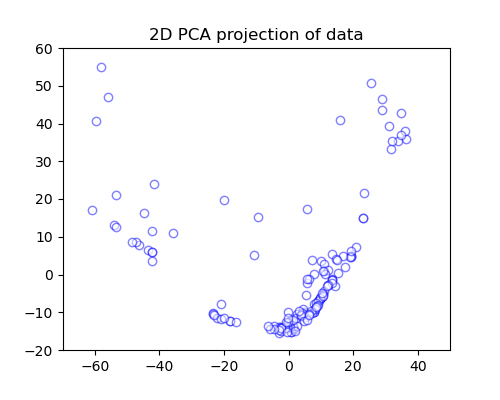
\includegraphics{q2_scatterplot}
	\end{center}
	

\section{Eigenfaces}
	\begin{enumerate}
		\item
			\begin{verbatim}
				See code in the Jupyter Notebook
			\end{verbatim}
	\end{enumerate}




\end{document}
